\iflanguage{ngerman}
{\chapter{Methoden und Umsetzung}}
{\chapter{Methods and Implementation}}
\label{sec:methods}

%design

This chapter describes the layout of the thesis' proposed solution. It also discusses implementation specifics and the tools used to build smart contracts and JASON \ac{BDI} agents. The \ac{BDI} agents work in a \ac{MAS} via JASON AgentSpeak and communicate via solidity and python-based smart contracts. We would talk about the application's design objectives and general overview. We will also go through the application's design and functionality for both creating smart contracts independently and after doing so, as well as for creating agents. We discuss the \ac{MAS} and \ac{BCT} implementation specifics, package and library versions utilized, and system configuration. Additionally, the procedures necessary to combine both in order to contribute to this thesis are also presented. This chapter's prerequisites include understanding the design and architecture of blockchain, AgentSpeak, and \ac{AOP} as described in the previous chapter. The prior chapter's contents should be reviewed in order to fully comprehend the chapters that follow.

\section{Roadmaps}

The initial roadmap will involve generating multiple agents in a \ac{MAS} and running them simply to see how they fulfill their objectives. Goals are the driving force that directs an agent's proactivity, as agents are expected to actively pursue the goals assigned to them without needing to be constantly stimulated, as opposed to object-orientation with service/method/function invocation, where services/objects are purely reactive entities that provide functionalities. Examine how agents summon each other by sending messages, as well as how they behave and interact with one another. 

\vspace{.5cm}

The next step will be to create smart contracts for each process on a blockchain, complete with state and events. Additionally, while creating the contract, select the appropriate language and version. After ensuring that everything is in order, combine \ac{MAS} and \ac{BCT} and try to run the overall program to ensure compatibility.

\section{Design Goals}

The purpose of this project is to develop an application that integrates \ac{MAS} and \ac{BCT}. To construct such an application, we took design considerations that influenced our architecture. We have certain particular goals in mind while contemplating integrating both technologies. The following design objectives are listed:
\vspace{.5cm}
\begin{itemize}

    \item \textbf{Decentralization} \\ One of the main advantages of using smart contracts and \ac{BDI} agents in supply chain management is that they allow for decentralized decision-making and coordination. The design of the system should aim to enable decentralized 

    \vspace{.5cm}
    
    \item \textbf{Autonomous} \\ To fulfill the objectives assigned to an agent, autonomy simply implies being able to work autonomously. An autonomous agent, thus, at the very least, makes independent judgments about how to accomplish its given goals; these decisions (and subsequently, its actions) are within its own control and are not influenced by other forces.

    \vspace{.5cm}

    \item \textbf{Transparency} \\ Smart contracts and \ac{BDI} agents are designed to provide transparency in the supply chain. The design of the system should aim to provide transparency of all activities and interactions among agents, allowing all parties to see the flow of goods and the state of the supply chain.

    \vspace{.5cm}
    
    \item \textbf{Efficiency} \\
    Effectiveness strategies improve the functioning of a smart contract or lower the expenses connected with its use. These patterns can help operators and consumers save time and money.
    
    \vspace{.5cm}

    \item \textbf{Interoperability} \\ The design of the system should aim for interoperability with other blockchain and non-blockchain platforms in order to enable the integration of existing systems and the exchange of information among different platforms.

    \vspace{.5cm}
    
    \item \textbf{Flexibility} \\
    Supply chains are complex and dynamic systems. The design of the system should be flexible enough to adapt to changing conditions in the supply chain. This can be achieved by programming the agents to reason and decide based on their beliefs, desires and intentions which can change over time.
    
    \vspace{.5cm}
    
    \item \textbf{Goal-directed behaviour} \\
    If an agent has been assigned a specific objective, it is assumed that the agent would attempt to attain the goal. Proactivity eliminates completely passive actors who never strive to accomplish anything.

    \vspace{.5cm}
    
    \item \textbf{Reactiveness} \\
    Implementing an application that achieves an appropriate mix of goal-directed and reactive behavior becomes difficult. This is one of the primary design goals of AgentSpeak.
    
    \vspace{.5cm}
    
    \item \textbf{Security} \\
    As \ac{MAS} on the blockchain will handle sensitive information, the security of the system is crucial. The design of the system should aim to protect agents and transactions from malicious actors.

    \vspace{.5cm}
    
    \item \textbf{Scalability} \\ As the number of agents and transactions in a supply chain increases, the scalability of the system can become a challenge. The design of the system should aim for scalability solutions that enable large-scale deployment of agent-based systems on the blockchain.
\end{itemize}

\section{System Configuration And Model Description}

The application is designed to be as basic as possible in order to learn how a supply chain works in the real world, i.e. each entity interacts with the other entity on a different level in order to complete the chain.

    \begin{figure}[h]
    \centering
      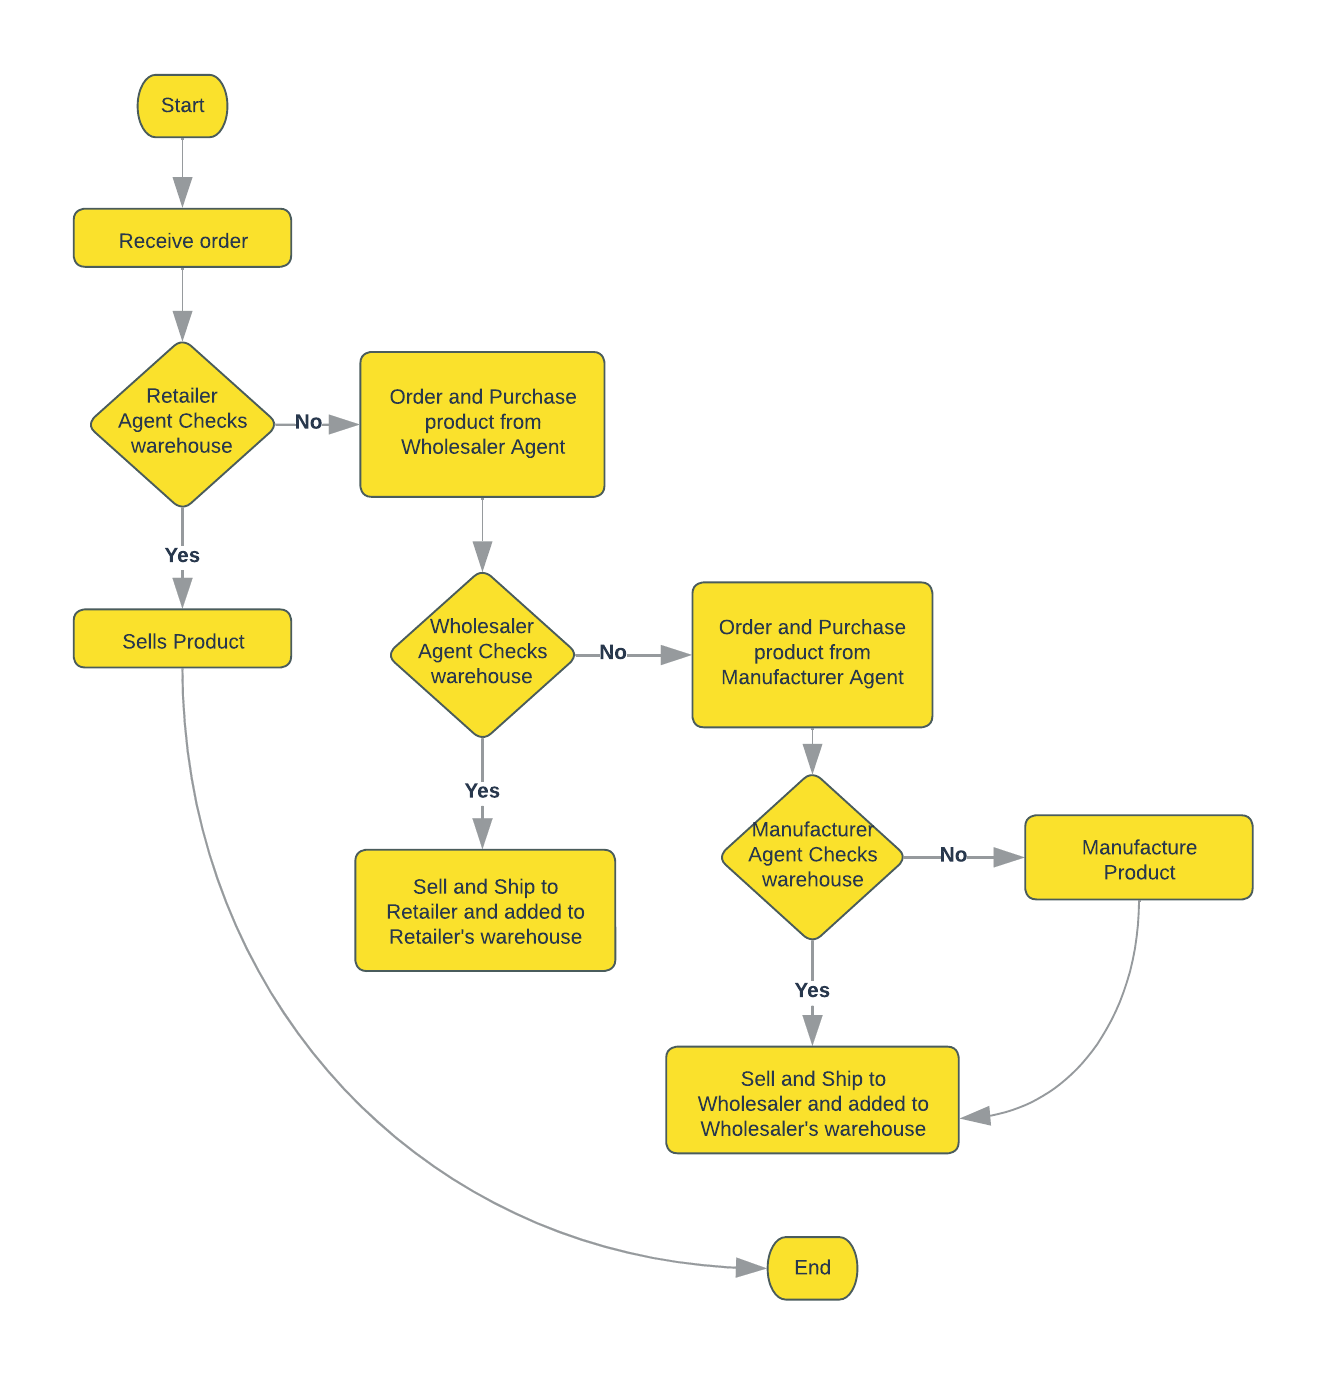
\includegraphics[width=10cm]{includes/figures/Flow Chart.png}
      \caption{Supply Chain Flow Chart}
      \label{Flow chart}
    \end{figure}

\vspace{.5cm}

The application flow for the \textit{Smart contract development with JASON \ac{BDI} agents} is depicted in Figure  \ref{Flow chart}. These three agents, a manufacturer, a wholesaler, and a retailer, each perform a specific function in the supply chain. All three of the other agents are being invoked by another primary agent in the \ac{MAS}. Figure \ref{Sequence Diagram} can be used for brief demonstration on which basis the contracts are to be created.

\vspace{.5cm}

   \begin{figure}[h]
    \centering
      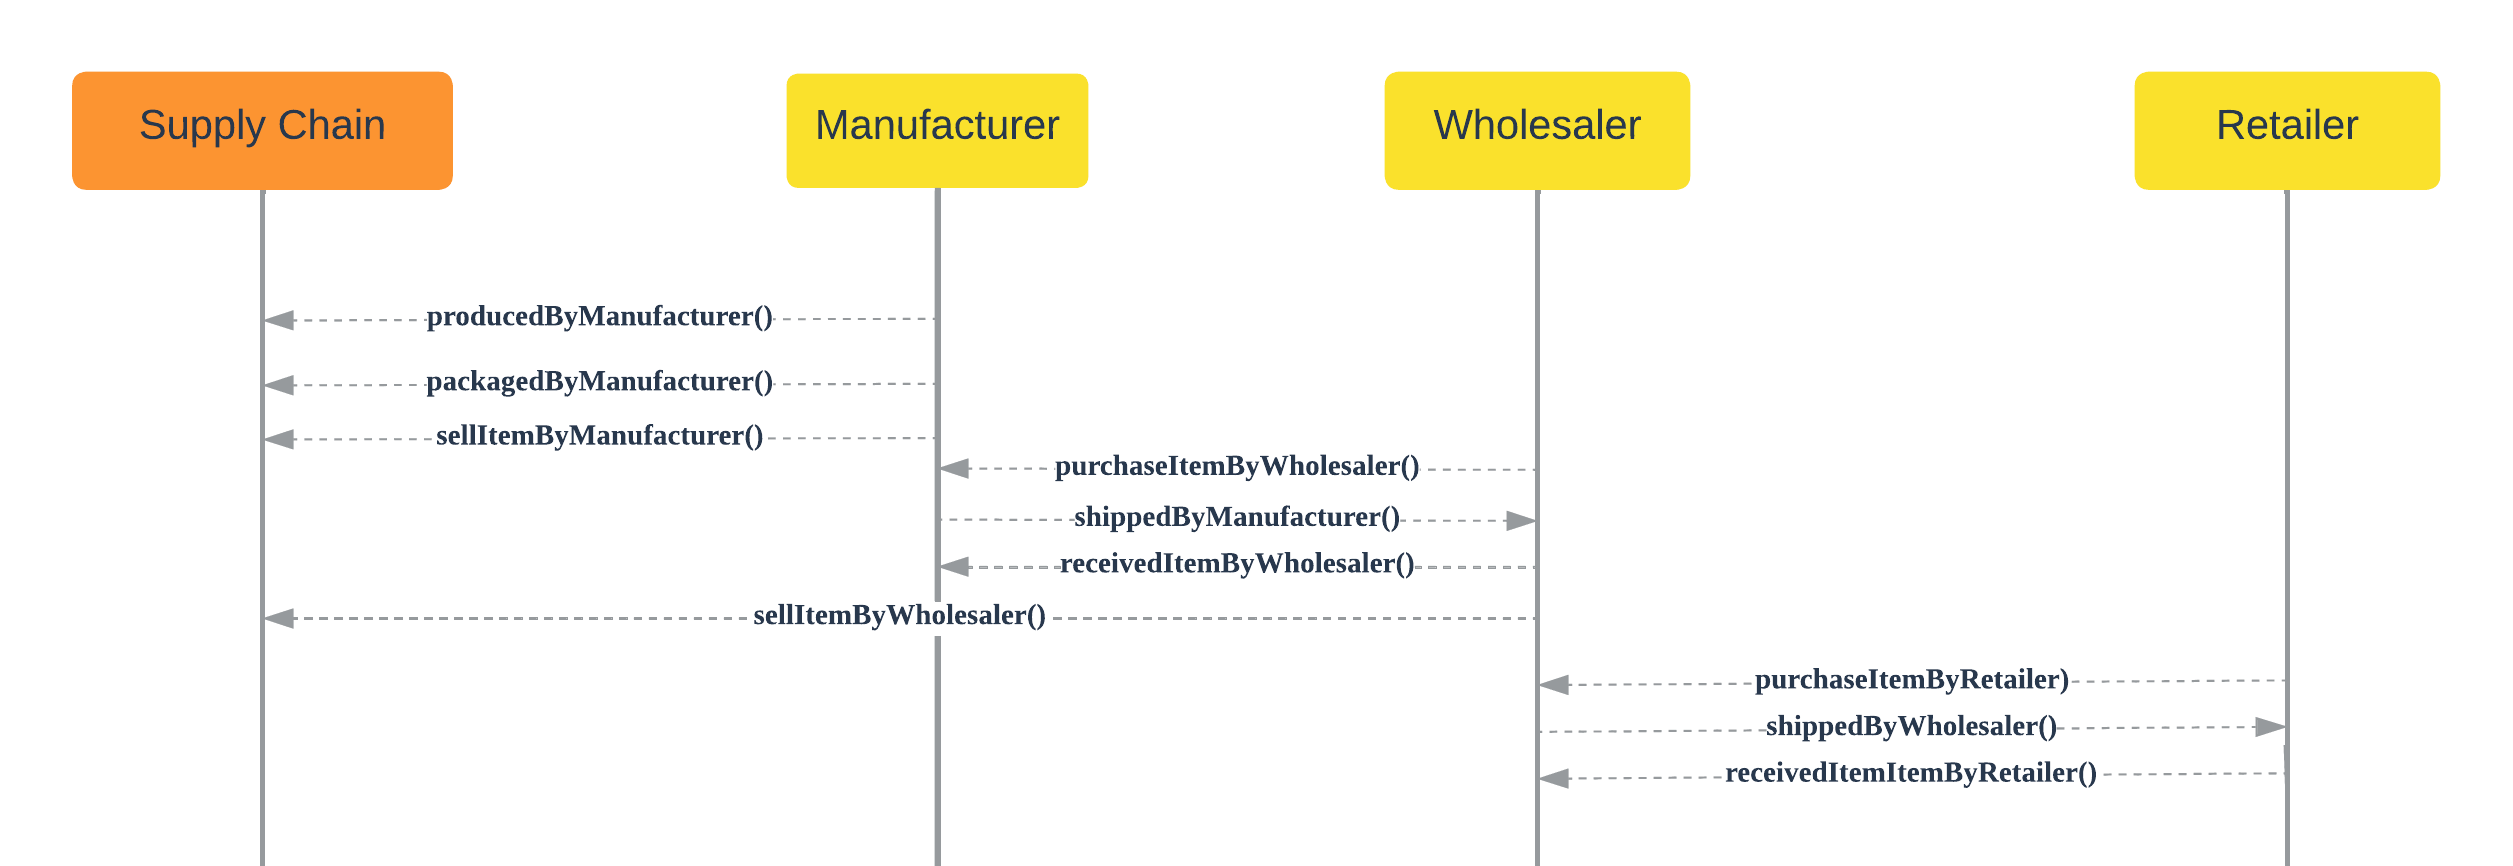
\includegraphics[width=\linewidth]{includes/figures/Sequence diagram.png} 
      \caption{State Sequence Diagram for Smart Contracts}
      \label{Sequence Diagram}
    \end{figure}

\vspace{.5cm}

The application was created and tested on a Linux Ubuntu 22.04.1 LTS system.
Visual Studio and InetlliJ are the \ac{IDE} used to create the application. \textit{jEdit} is also used somehow to run agents using JASON while creating \texttt{.asl} and running \texttt{.mas2j} file.
To test the compatibility of web3j with gradle for agents, many versions of Java Standard Edition Development Kit were utilized, however the most commonly used was Java SE Development Kit 18.0.2.1. 

\vspace{.5cm}

Other standards for the development of Smart contracts and agents are detailed in the sections below.

\section{Smart Contracts Development }   

While taking into consideration the scenario of a supply chain where all information on suppliers, recipients, products, and business circumstances is dispersed over supply chain databases.
It is possible to execute the sale of products or services as a transaction that is cryptographically signed by the seller and the buyer and attached to a smart contract for sales transactions. When the sale occurs and all other conditions, such as documentation and quality checks, are met, the execution of the transfer of the corresponding funds and rights can be enforced; in other words, smart contracts can ensure that collaborative and entrepreneurial processes are carried out correctly.

\vspace{.5cm}

As aforementioned, the terminology blockchain refers to two things: a distributed database and a data structure (i.e. a linked list of blocks containing transactions, where each block is cryptographically chained to the preceding one by incorporating their hash value and a cryptographic signature, in such a manner that changing an earlier block requires re-creating the whole chain since that block). The idea of smart contracts, which are scripts that run every time a specific kind of transaction takes place and may read and write to the blockchain, is related to the blockchain technology. Smart contracts enable parties to enforce the requirement that while one transaction occurs, other transactions also occur.

\vspace{.5cm}

    \begin{figure}[h]
    \centering
      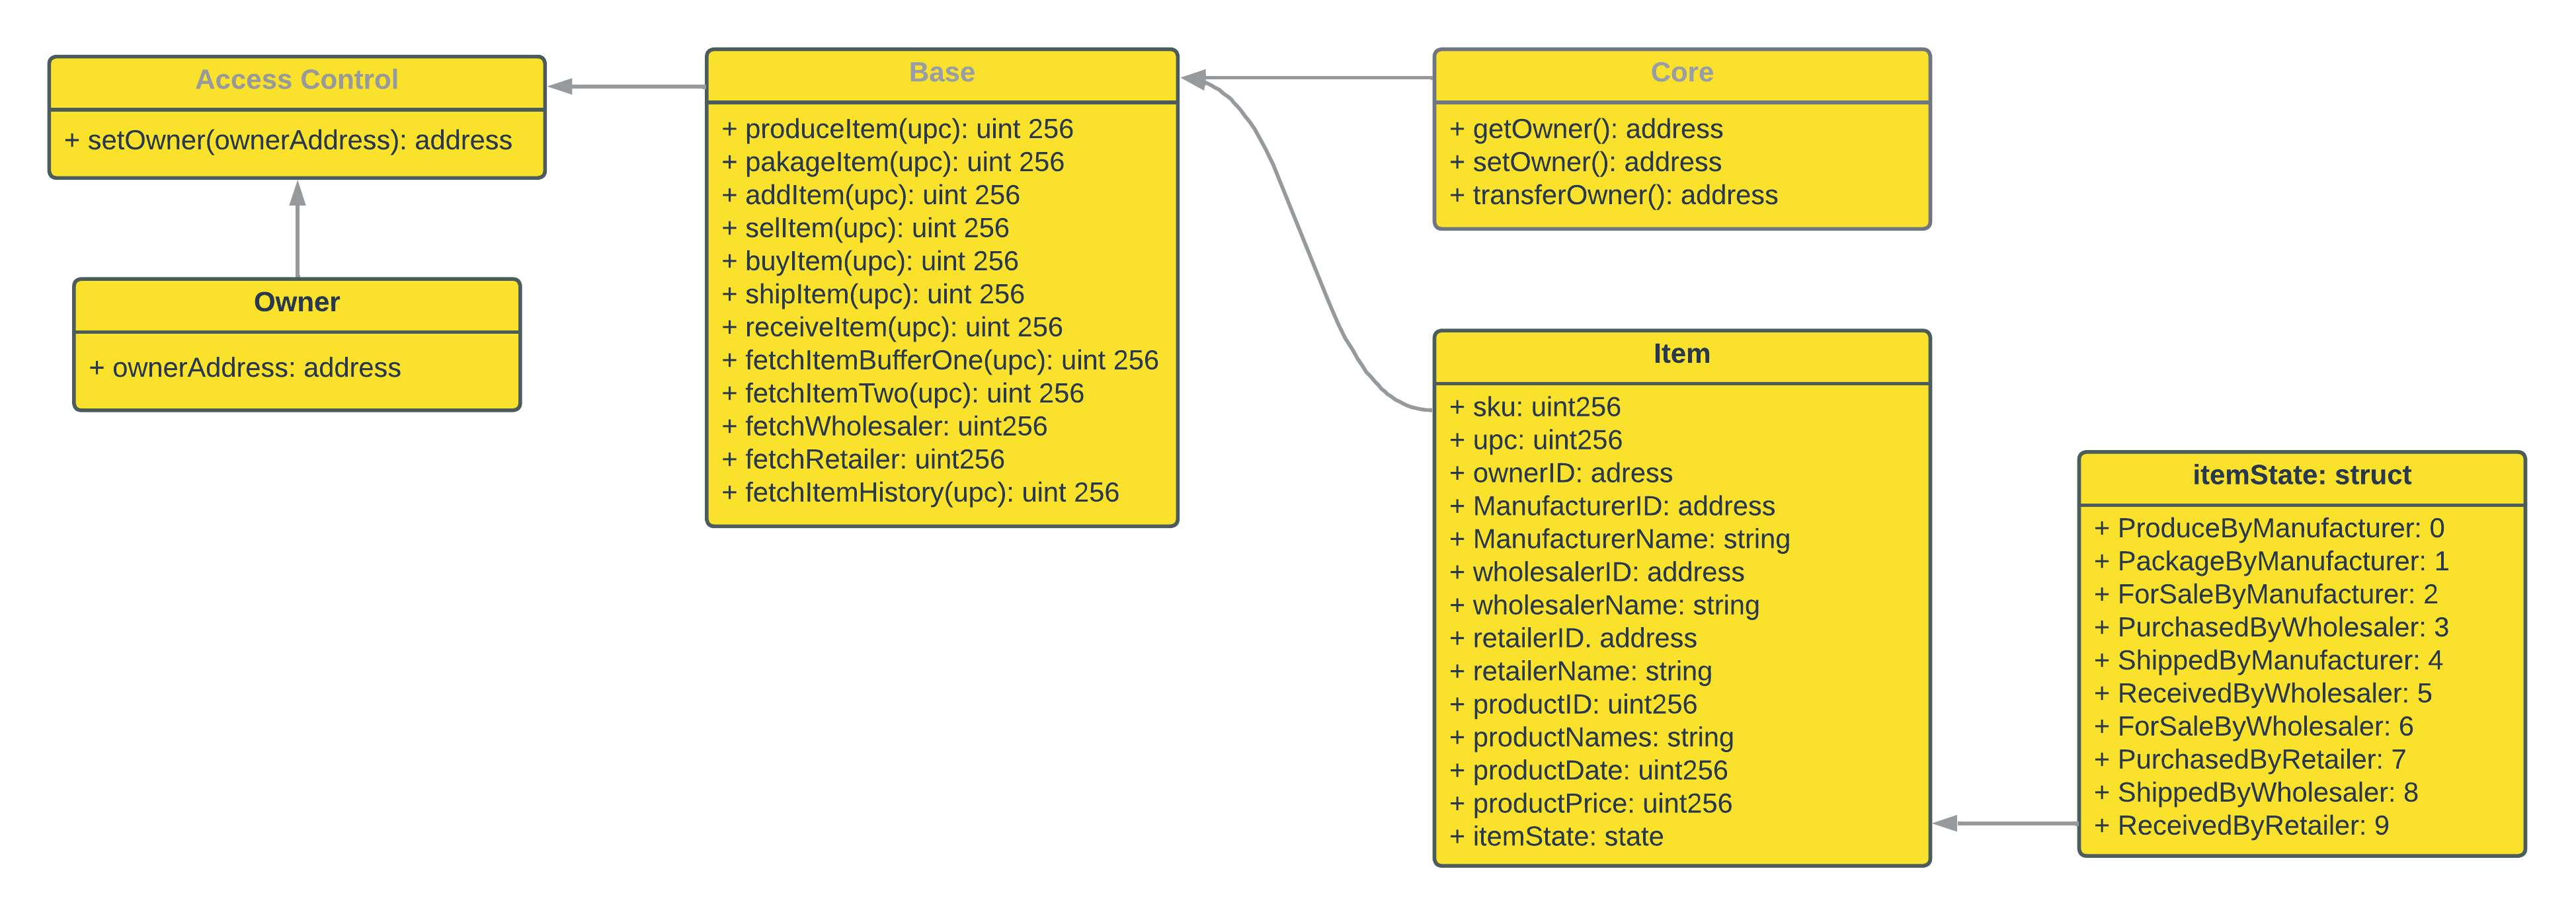
\includegraphics[width=15cm]{includes/figures/Data Model diagram.png} 
      \caption{Smart Contract's Data Model Diagram}
      \label{Data Model diagram}
    \end{figure}
    
\vspace{.5cm}

The programming for smart contracts related supply chain is done using Solidity Language while keeping the version in mind in order to integrate it with the agent programming language so that they can work together. Smart contracts perform the following functions: (1) The product is produced by the manufacturer, (2) the manufacturer completes the packaging, (3) the product is placed on the market, (4) the wholesaler purchases the product, (5) the manufacturer ships the product, (6) the wholesaler receives the product, (7) the wholesaler places the product on the market, (8) the retailer purchases the product, (9) the wholesaler ships the product, and (10) the retailer receives the product as the final result.

\vspace{.5cm}

Each function is regarded as an event, and every event is given a state, as shown in Figure \ref{Data Model diagram}. It has always been a rule that each event must occur after the one before it has concluded. For example, a manufacturer cannot sell a product before producing it, while a wholesaler cannot receive a product before buying it. It is carried out with the aid of a state check. A product can also be tracked using the \ac{UPC} or by utilizing the \ac{SKU} to trace the entire batch.

\vspace{.5cm}

Solidity language is used to create smart contracts, while JavaScript is used for testing. The \texttt{.sol} files were compiled using Solidity v0.8.13, which also produced \texttt{.abi} and \texttt{.bin} files. The truffle tool, especially truffle v5.6.5, has been used for deployment and testing. We have used ganache v7.5.0 and ganache-UI v2.5.4 to examine state and manage chain behavior. All of the packages listed below have been obtained using node v14.0.0 (npm v6.14.4) in the table \ref{Package Version}.
    
\vspace{.5cm}

\begin{table}[h]
\small
\centering
\caption{Package Version}
\label{Package Version}
\begin{tabular}{|l| l|}
\hline
\textbf{Node Package} & \textbf{Version} \\ 
\hline\hline
web3 & 1.7.5\\ \hline
truffle & 5.6.5\\ \hline 
@truffle/contract & 4.5.22\\ \hline 
@truffle/hdwallet-provider & 2.0.13\\ \hline
dotenv & 16.0.1\\ \hline
geth & 0.4.0\\ \hline
openzeppelin & 4.7.3\\ \hline
\hline 
\end{tabular}
\end{table}

\vspace{.5cm}

Figure \ref{Activity Diagram} was used as a reference for developing smart contracts connected to supply chain. The following events were included in the supply chain: To complete the supply chain, (i) the manufacturer manufactures the product, (ii) the manufacturer packages the product, (iii) the manufacturer sells the product to the wholesaler, (iv) the wholesaler purchases the product, (v) the wholesaler receives the product, (vi) the wholesaler sells the product to the retailer, (vii) the retailer purchases the product, (viii) the retailer receives the product, and restocks his/her inventory.

\vspace{.5cm}

\begin{figure}[h]
\centering
  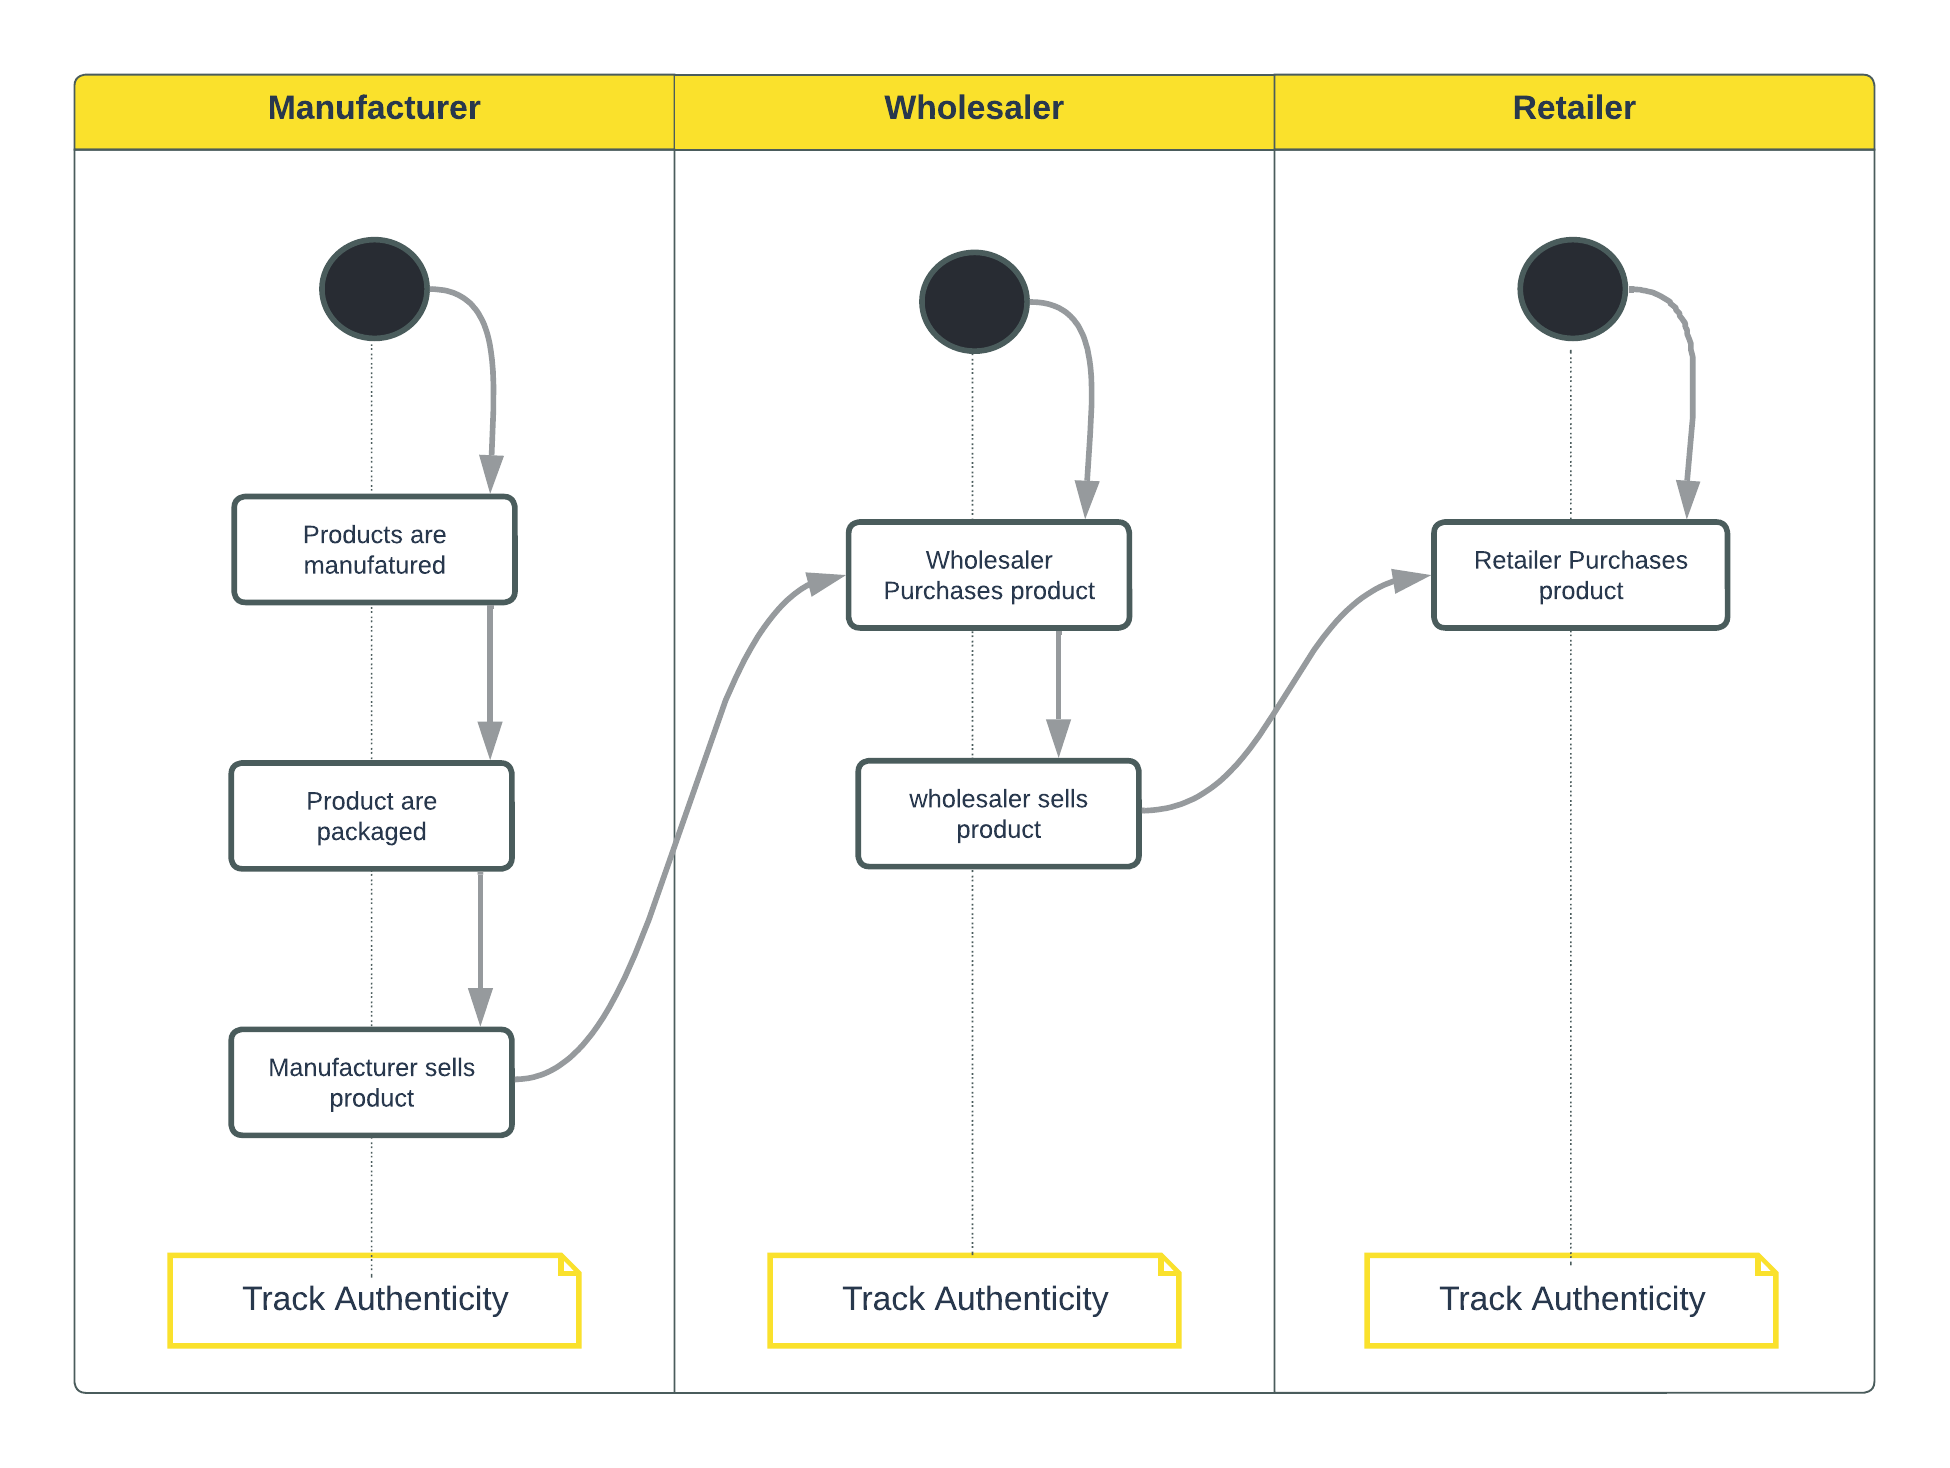
\includegraphics[width=12cm]{includes/figures/Activity Diagram.png} 
  \caption{Supply Chain Activity Diagram}
  \label{Activity Diagram}
\end{figure}

\vspace{.5cm}

The way in which files organised an classes imported using inheritance can be understand from Figure \ref{Data Model diagram}, but for the in depth understanding Figure \ref{Overall Class Diagram} should be taken into consideration. Solidity contracts can make use of a particular type of remark to give detailed documentation for functions, return variables, and other features. The name of this unique format is the \ac{NatSpec}. The formatting for comments used by the author of a smart contract and recognized by the Solidity compiler is included in \ac{NatSpec}. Additionally, third-party tool annotations may be included in \ac{NatSpec}. The \texttt{@custom:<name>} tag is most likely how they are completed, and analysis and verification tools are an excellent example of this in usage.

\vspace{.5cm}

\textbf{Vyper} was also chosen to construct smart contracts, which is now one of \ac{DeFi}'s most popular languages. Vyper is a high-level programming language identical to Python. However, due to its limitations over Solidity, the proposal was subsequently abandoned.


\begin{figure}[!h]
\centering
  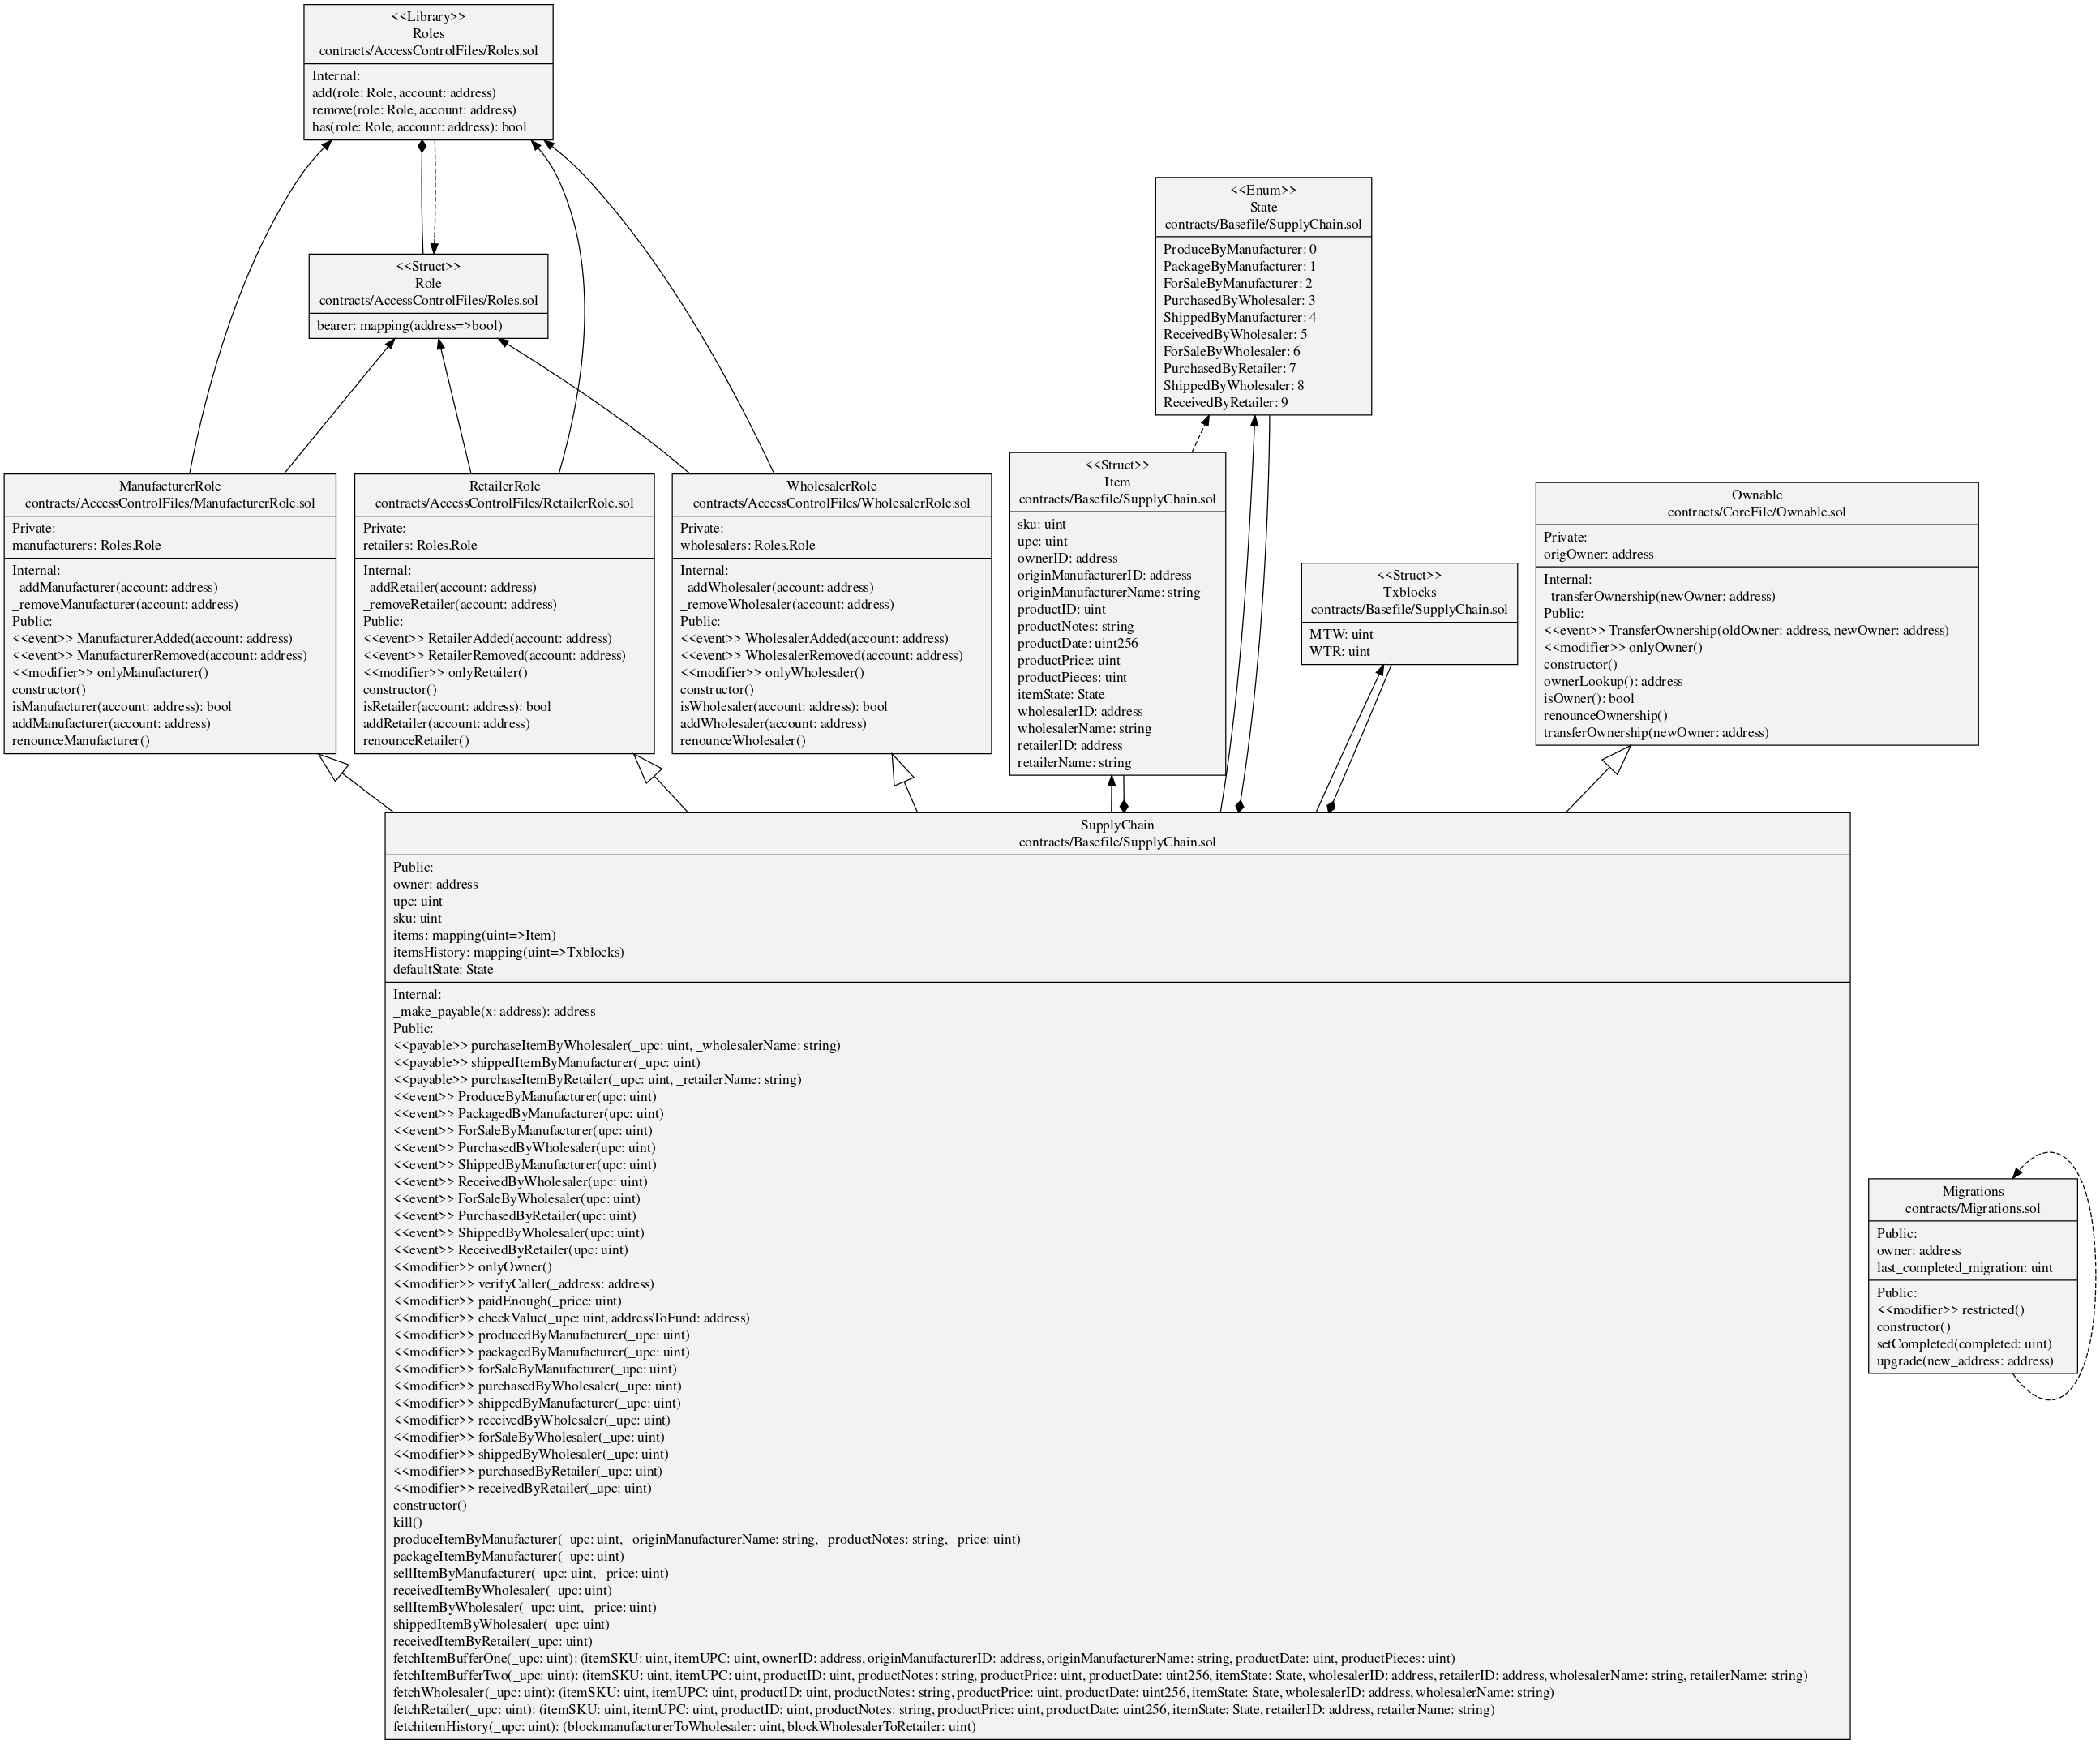
\includegraphics[width=21cm, angle=90]{includes/figures/OverallClassDiagram.png} 
  \caption{Smart Contract Class Diagram}
  \label{Overall Class Diagram}
\end{figure}


\section{Agent Model Implementation}

An agent continually perceives its environment, makes decisions about how to act to achieve its objectives, and then takes action to alter the surroundings. The speech-act theory is commonly used to describe agent communication in \ac{MAS}. The speech-act hypothesis is based on the premise that language is action.

\vspace{.5cm}

\begin{figure}[h]
    \centering
      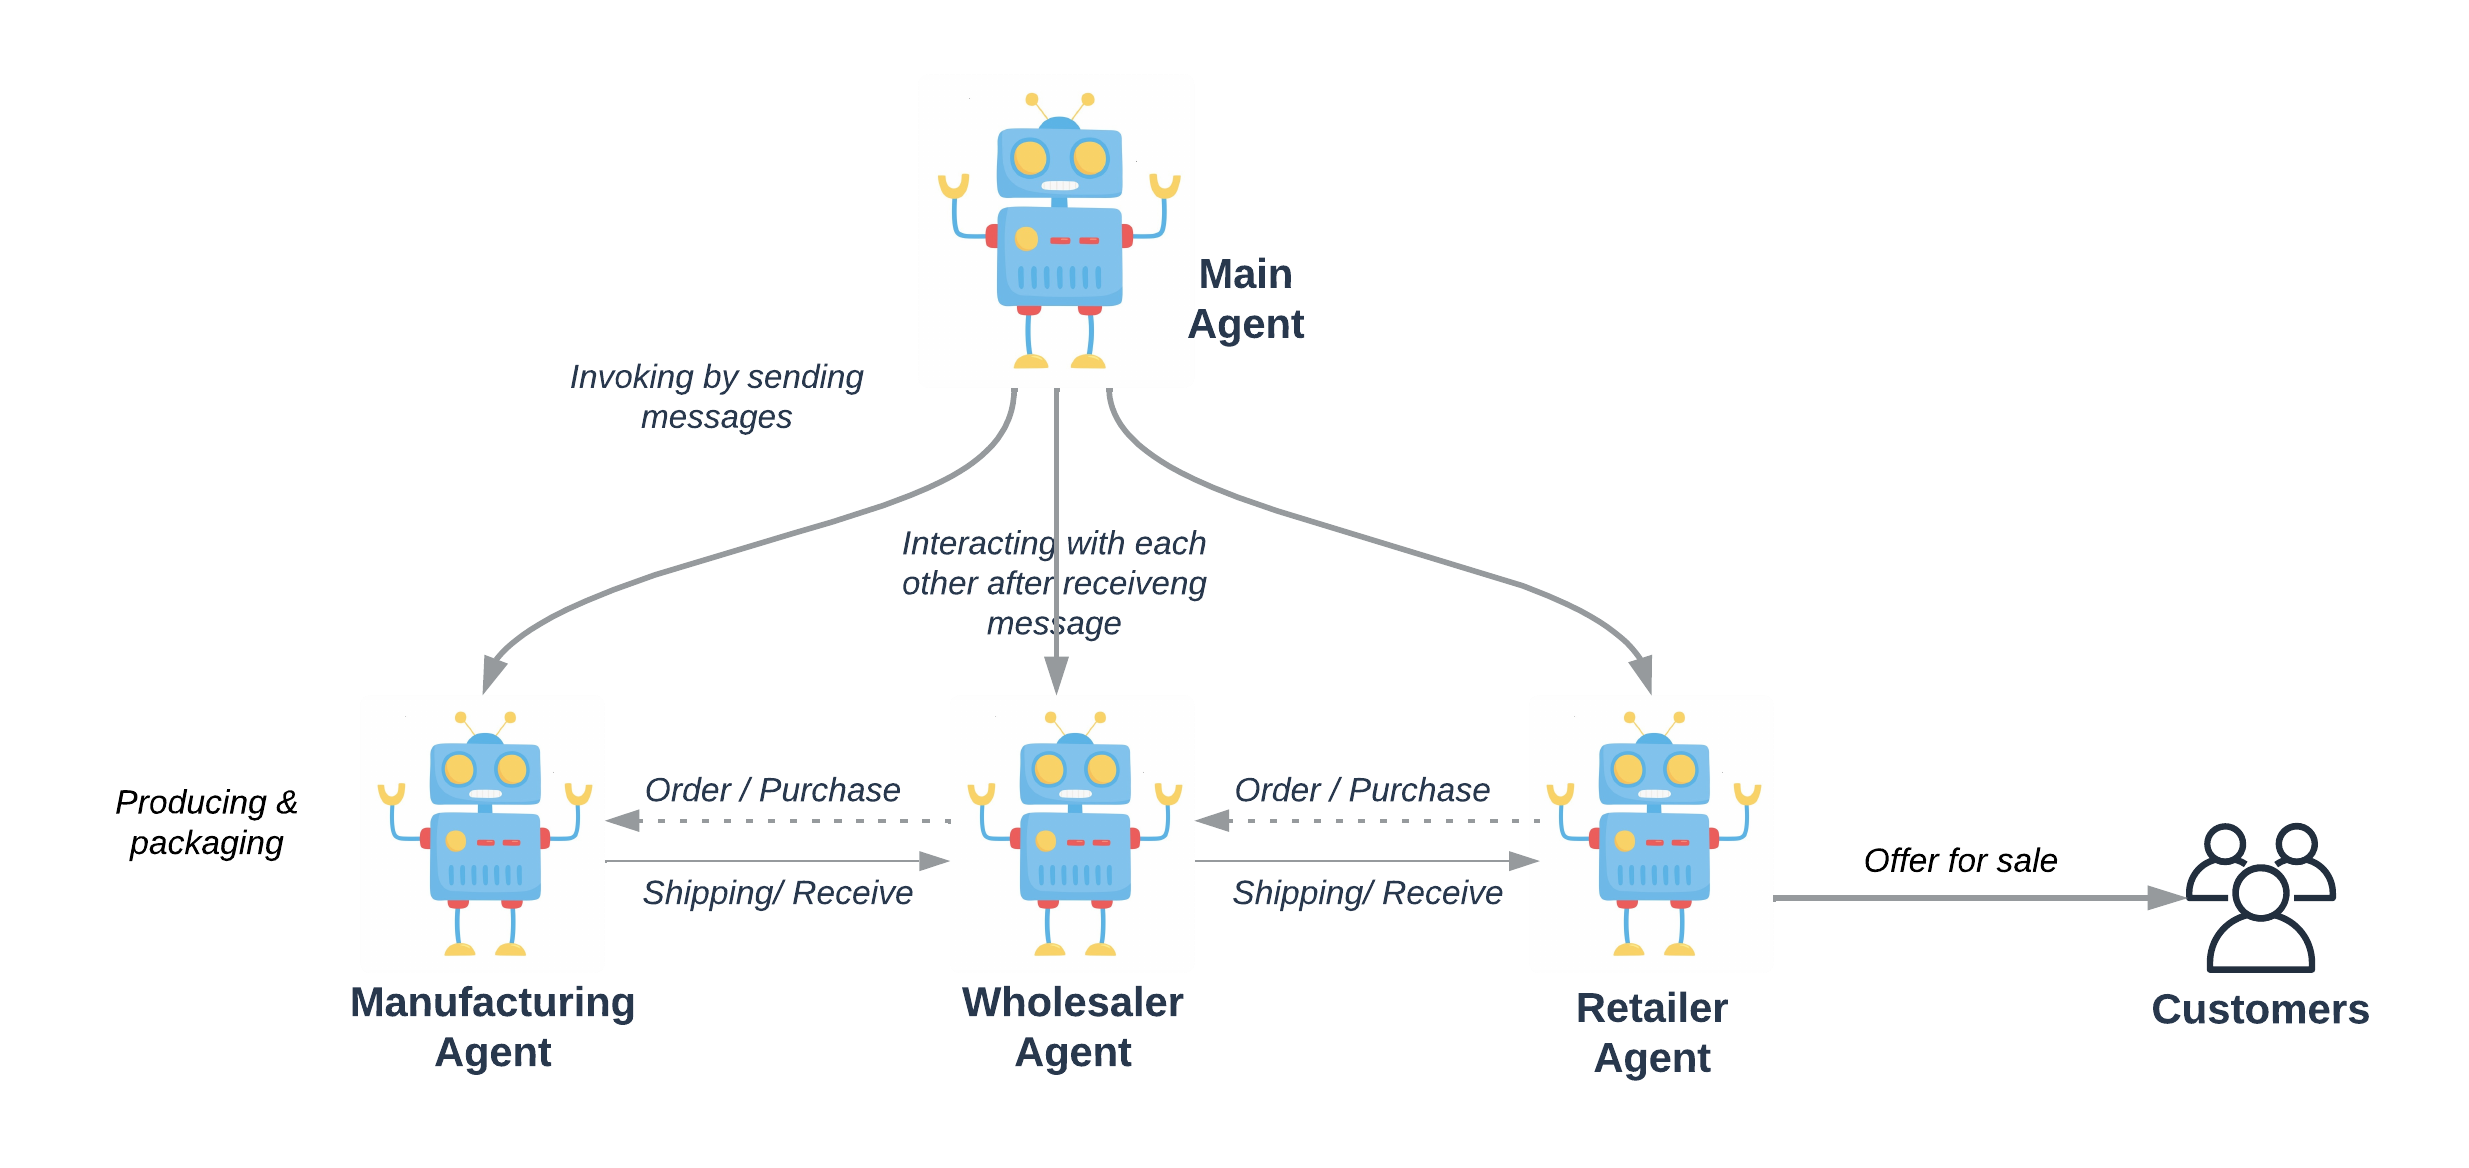
\includegraphics[width=\linewidth]{includes/figures/agent.png} 
      \caption{Agent Interaction in Supply chain}
      \label{Agent Interaction}
    \end{figure}
  
\vspace{.5cm}

An agent program is run by the JASON interpreter. An agent uses a reasoning cycle to carry out its operations, which may be broken down into the following steps: first, it perceives the environment; second, it updates the belief base; third, it receives communication from other agents; fourth, it selects "socially acceptable" messages; fifth, it chooses an event; sixth, it retrieves all relevant plans; seventh, it determines the applicable plans; eighth, it chooses one applicable plan; and last, it executes one step of an intention.

\vspace{.5cm}

In our \ac{MAS}, each participant's function within the supply chain will be handled by an agent , see Figure \ref{Agent Interaction}. The retailer agent will work to ensure that the product is available in the warehouse before ordering it from the wholesaler agent, who will then ask the wholesaler to check its inventory, get in touch with the manufacturer to produce the product, and ship it to the wholesaler, who will then send it to the retailer agent. There will be a \textit{main agent}, who will launch the retailer agent's efforts to sell items to consumers and also other agents by sending messages.

\vspace{.5cm}

The \ac{BDI} architecture is the most common technique to implementing "intelligent" or "rational" agents. The specification of a set of base beliefs and a set of plans results in the creation of an AgentSpeak(L) agent. AgentSpeak(L) differentiates between two kinds of goals: achievement goals and test goals. However, we use achievement targets for our agents. We employed a variety of techniques while writing our agents and ensuring that they could be utilized with smart contracts. We tested several different interpreters and wrote our agents using those. We pursue the following strategies:

 \vspace{.5cm}
 
\begin{itemize}
    \item \textbf{JASON (Java-based interpreter)}
    
    \vspace{.5cm}
    
    \item \textbf{\ac{ASTRA}}
    
    \vspace{.5cm}
    
    \item \textbf{JASON (Python-based interpreter)}
    
     \vspace{.5cm}
\end{itemize}

The solutions listed above have been defined later in this chapter.

\vspace{.5cm }

The structure of the agent program is governed by the fact that there will be four agents in the \ac{MAS}, as shown in Figure \ref{Agents in MAS} in MAS, and they will interact with each other as shown in Figure \ref{Agent Interaction}. Our implementation strategy is as follows:

\begin{itemize}
    \item The supply chain will be initiated by the main agent, who will then engage the retailer agent;
    
    \vspace{.5cm}
    
    \item Retailer agent will inspect its inventory and sell products to customers; if a product is not in stock, retailer agent will ask the main agent to contact the wholesaler agent;
    
    \vspace{.5cm}
    
    \item The wholesaler agent will check its warehouse and ship the product to the retailer agent; if the product is not available, the wholesaler agent will request that the manufacturer agent be contacted by the main agent;
    
    \vspace{.5cm}
    
    \item Upon checking its inventory, the manufacturer agent will ship the product to the wholesaler agent. If the product is not in stock, the manufacturer agent will manufacture the product, does the package and deliver it to the wholesaler.
    
    \vspace{.5cm}
    
\end{itemize}

Every implementation uses the same approach to how agents cooperate and communicate, and each implementation is detailed in more detail in the section below.

\begin{figure}[h]
\centering
  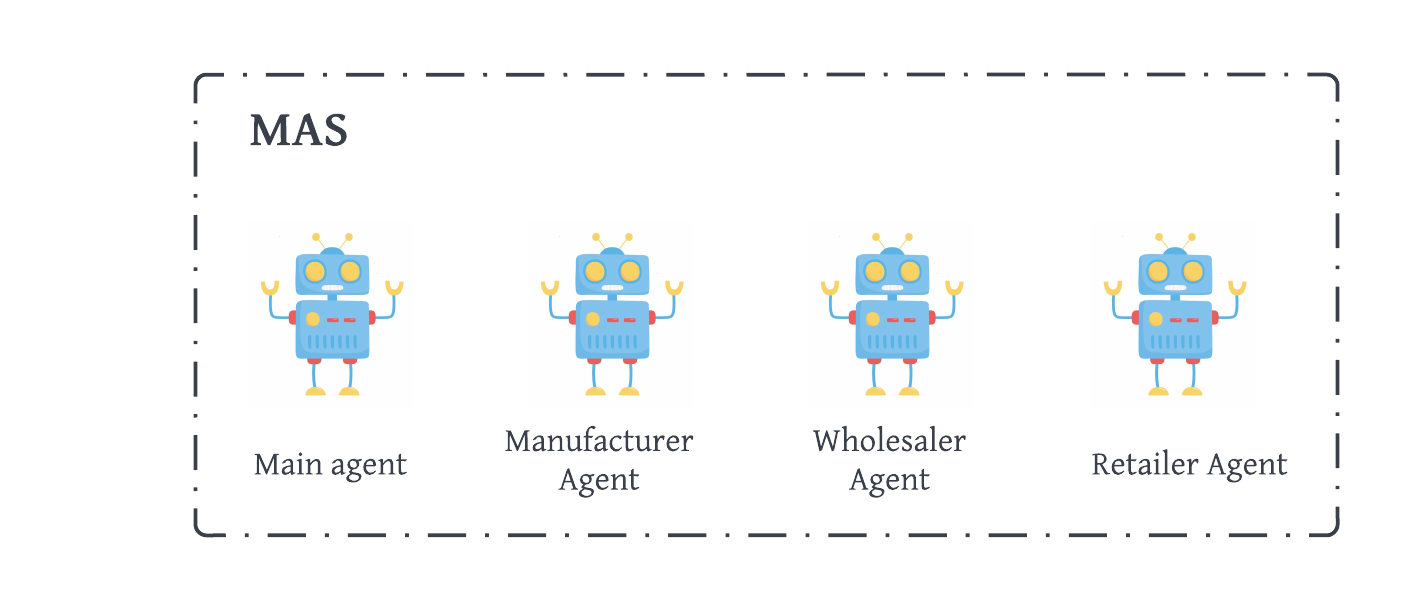
\includegraphics[width=10cm]{includes/figures/MAS.png} 
  \caption{Agents in \ac{MAS}}
  \label{Agents in MAS}
\end{figure}

\subsubsection{JASON (Java-based interpreter)}

We first used JASON with a Java-based interpreter to develop the agents in \ac{MAS}. We set up the home variables, downloaded the necessary scripts and libraries, then used gradle as well as maven for simple configuration. AgentSpeak's expanded dialect has an interpreter named JASON. It implements the operational semantics of that language and offers a platform for creating \ac{MAS} with a variety of characteristics that may be altered by the user. Version 3.1 of JASON, which is the most recent version, was installed. The agents are constructed using figure  \ref{Agent Interaction} as a guide.

\vspace{.5cm}

In addition to being able to interpret the original AgentSpeak, JASON possesses a few other crucial abilities. Inter-agent communication based on speech acts and strong negation are included, allowing for the use of both closed- and open-world assumptions. Additionally, it supports creating environments (which are not normally to be programmed in AgentSpeak; in this case they are programmed in Java). It offers the ability to deploy distributed \ac{MAS} via a network (using \ac{JADE}); the user may also add other distribution infrastructures. Furthermore, it offers an \ac{IDE} in the form of an Eclipse or jEdit plugin; the \ac{IDE} has a "mind inspector" that aids with debugging.

\subsubsection{ASTRA Implementation}

\ac{ASTRA} programs are divided into agent classes, which may be expanded using a multiple inheritance paradigm. Each agent class is written in a separate file with the same name as the agent class and the \texttt{.astra} extension. \ac{ASTRA} is distinct from AgentSpeak (L). Because \ac{ASTRA} applications can refer to Java classes, support for delivering fully qualified class names is required. \ac{ASTRA} programs incorporate partial plans (called plan bodies) in addition to plan rules to promote code/class resuability. \ac{ASTRA} strives to be familiar to developers who are familiar with mainstream programming languages, particularly Java.

 \vspace{.5cm}
 
Agent Programming Languages are intended to aid in the creation of \ac{MAS}. Such systems are intended to have more than one agent and more than one agent type by default. Support for deploying numerous agents is given in many Agent Programming Languages via deployment files, which let the developer to define the initial community of agents to be deployed. \ac{ASTRA} does not support this; instead, you construct an agent that generates new agents. The System \ac{API} provides the essential functionality to allow this approach. In \ac{ASTRA}, coding one agent to produce another agent is extremely straightforward. You just invoke the System \ac{API}'s \texttt{createAgent(...)} operation.

\subsubsection{JASON (Python-based interpreter)}

An interpreter for JASON, an agent-oriented programming language, built on Python. It can be installed in the system using \texttt{\ac{pip}}. For our implementation, we utilized agentspeak 0.1.0. Python-agentspeak is similar to JASON, except you don't need to create a \texttt{.mas2j} file to construct a multi-agent system; instead, all the agents may be called together by calling them in a \texttt{.py} file.


\section{Agent-Contract Collaboration}

 
 We are largely focused on agent-oriented models and technology, and we have smart contracts directly incorporated into the blockchain. With reference to the illustration \ref{Agent Interaction}, the model will be the same for the agents, but their communication will take place via smart contracts, be recorded as transactions on the blockchain, and be subsequently verified using the transaction hashes.
 
 \vspace{.5cm}

The thesis' core premise is the integration of the two technologies, \ac{MAS} and \ac{BCT}. We have tried to integrate both the technologies using several tries by using several web3 libraries, i.e., \textit{web3.js} for JavaScript, \textit{web3.py} for Python and \textit{web3j} for Java in order to interact with Ethereum.

\subsubsection{JASON and Web3j}

We attempted to test each smart contract using web3js after generating them with Solidity. We considered migrating to web3j since it would be simpler as opposed to continuing to utilize JASON AgentSpeak, which is based on Java. Through the Command Line Tools tool, Web3j facilitates the development of Java smart contract function wrappers from Solidity ABI files or straight from Truffle's Contract Schema. To reveal the contract's per-network deployment address, a wrapper is "improved" and produced. When the wrapper is created, these addresses are from the truffle deployment.

\vspace{.5cm}

The plan to utilize Web3j with JASON was eventually scrapped since, in order for JASON to run \ac{MAS}, the \texttt{.mas2j} file had to be executed, and when it did, it couldn't find the \texttt{org.web3j} package. We attempted to download the jar files locally, change the version of web3j and JASON, and switched from gradle to maven in order to make the program run, but the problem persisted.

\subsubsection{ASTRA and Web3j}

After several attempts with web3j and JASON, we considered switching to \ac{ASTRA}, a programming language that is quite similar to Java and aims to be familiar to developers with language. A successful agent construction was followed by the same problem as with JASON when importing the web3j package.

\subsubsection{JASON and Web3.py}

Web3.py is a Python package that allows you to connect with Ethereum. It is often used in \ac{Dapp}s to support a number of use cases, including sending transactions, communicating with smart contracts, accessing block data, and more. The Web3.js JavaScript \ac{API} served as the foundation for the original \ac{API}, which has since expanded to meet the demands and conveniences of Python developers.

\vspace{.5cm}

JASON's Python interpreter and Web3.py worked well together. In order to communicate or convey messages from one agent to another, \texttt{.asl} files for agents were produced in Python using AgentSpeak, which is a bit different from JASON constructed using Java. Additionally, running a \texttt{.mas2j} file is not necessary for \ac{MAS} in JASON-style AgentSpeak for Python.

\subsubsection{JASON and Jython}


Jython is a Python programming language implementation meant to operate on the Java platform. JPython was the previous name for the implementation. Any Java class may be imported and used by Jython apps. Jython applications, with the exception of a few common modules, employ Java classes rather than Python modules. 

\vspace{.5cm}
Jython provides practically all of the modules found in the standard Python programming language package, with the exception of a few modules written in C. Jython either dynamically or statically converts Python source code to Java bytecode (an intermediate language). The following tasks are especially well suited for Jython:

\begin{itemize}
    \item In order to interact with Java packages or run Java programs, Jython provides an interactive interpreter. This makes it possible for developers to experiment with and debug any Java system using Jython.
    \vspace{.5cm}
    \item Users can write simple or intricate scripts using embedded scripting to increase an application's capabilities. The Jython libraries are available to Java programmers for their systems.
    \vspace{.5cm}
     \item Python scripts are frequently 2–10 times shorter than their Java equivalents, enabling quick development of applications. This has a direct impact on how efficiently programmers work. Python and Java get along well with one another, allowing programmers to mix the two languages at will during both product development and release.
\end{itemize}

\vspace{.5cm}

JASON AgentSpeak's smart contract development for Python and Web3.py was a success that we explained in the next chapter. So we decided to give it another shot and try to develop it using Jython. The Jython project provides Python implementations in Java, giving Python the benefits of operating on the JVM and access to Java classes.

\vspace{.5cm}

The next chapter explains the results from our suggested approaches for taking the steps along smart contracts deployed in a bespoke blockchain with their own flow of control among agents constructed utilizing agent oriented language.

